\chapter{Projeto do Sistema} \label{cap:projeto}

Este capítulo estabelece a especificação técnica da solução \textbf{Karaokê Apache}, transformando o modelo conceitual e os requisitos da análise em uma definição detalhada da arquitetura distribuída, dos componentes de software, do modelo lógico e físico de dados, do projeto das interfaces de usuário, das interações dinâmicas, das tecnologias adotadas e dos mecanismos de segurança.

\section{Arquitetura do Sistema}

A arquitetura do sistema \textbf{Karaokê Apache} foi elaborada a partir dos artefatos de engenharia \texttt{ideia.png} e \texttt{Desenho da Aplicação}, estruturando a solução em quatro subsistemas integrados: \textbf{Cliente Web}, \textbf{Admin Web}, \textbf{API Orquestradora} (conectada ao \textbf{Banco de Dados Relacional}) e o reprodutor desktop \textbf{Electron (Karaokê TV Player)}.

Seguindo os princípios de desacoplamento arquitetural descritos por Sommerville \cite{sommerville2019}, Fowler \cite{fowler2006} e Pressman e Maxim \cite{pressman2016}, a camada de apresentação web e o reprodutor de telão permanecem separados da lógica de persistência, comunicando-se por meio de contratos bem definidos. Na modelagem formal realizada pela equipe na ferramenta UMLet (arquivos \texttt{diagrama\_de\_componentes.uxf} e \texttt{diagrama\_de\_componentes.png}), a arquitetura lógica é organizada em quatro componentes principais (\textbf{Usuários}, \textbf{Fila}, \textbf{Pedido de Música} e \textbf{Reprodutor}), representados no \textbf{Diagrama de Componentes UML} da Figura \ref{fig:uml_componentes}.

\begin{figure}[H]
  \caption{Diagrama de Componentes UML (\texttt{diagrama\_de\_componentes.png}).}
  \label{fig:uml_componentes}
  \begin{center}
    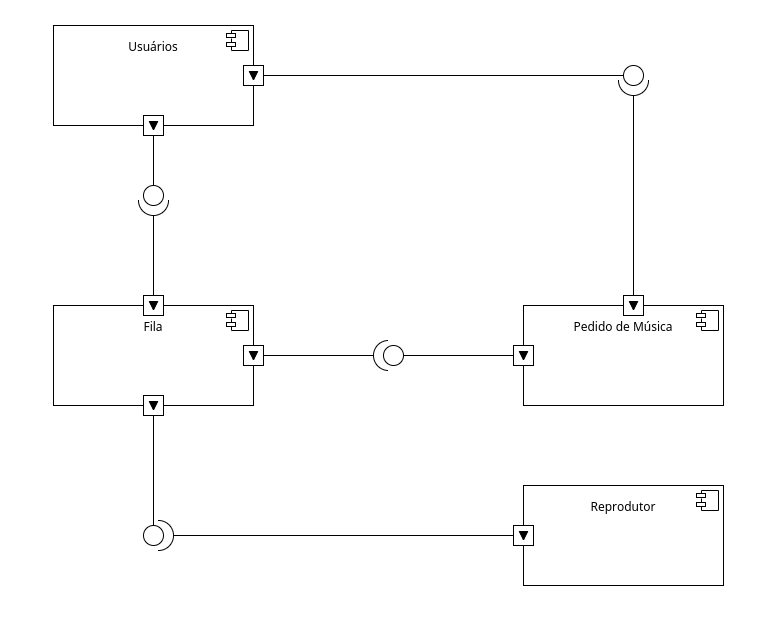
\includegraphics[width=0.88\textwidth]{imagens/diagrama_de_componentes.png}
  \end{center}
  \legend{Fonte: Elaborado pelos autores no software UMLet (2026).}
\end{figure}

\section{Projeto dos Componentes}

Cada componente definido na arquitetura possui responsabilidades coesas e interfaces explícitas de comunicação, detalhadas na Tabela \ref{tab:componentes_uml}:

\begin{table}[H]
\IBGEtab{%
  \caption{Detalhamento técnico dos componentes arquiteturais e suas interfaces.}%
  \label{tab:componentes_uml}%
}{%
  \footnotesize
  \begin{tabularx}{\textwidth}{p{3.0cm}p{4.2cm}X}
    \toprule
    \textbf{Componente} & \textbf{Interfaces (Fornecidas / Requeridas)} & \textbf{Estrutura Interna e Responsabilidades} \\
    \midrule
    \texttt{Usuários} & Fornece: \texttt{IAutenticacao}, \texttt{IPerfilUsuario} & Responsável pelo cadastro, autenticação e diferenciação de permissões entre os papéis \texttt{cliente} (frequentador da mesa) e \texttt{admin} (organizador do palco). \\
    \addlinespace
    \texttt{Pedido de Música} & Requer: \texttt{IAutenticacao}; Fornece: \texttt{IPedidoMusica} & Responsável pela pesquisa e escolha de vídeos musicais diretamente pelo sistema, identificação do vídeo selecionado e validação de disponibilidade (RN00). \\
    \addlinespace
    \texttt{Fila} & Requer: \texttt{IAutenticacao}, \texttt{IPedidoMusica}; Fornece: \texttt{IControleFila} & Núcleo orquestrador do sistema: gerencia a lista ordenada de pedidos (\texttt{queue}), o item em execução (\texttt{currentSong}), aplica o bloqueio de duplicidade (RN01) e processa os comandos \textit{Play}, \textit{Próxima}, \textit{Remover} e \textit{Limpar}. \\
    \addlinespace
    \texttt{Reprodutor} & Requer: \texttt{IControleFila} & Materializado pelo aplicativo desktop \textit{Karaokê TV Player} em Electron: escuta continuamente o estado de \texttt{currentSong} e atualiza o player embarcado em tela cheia na TV do bar. \\
    \bottomrule
  \end{tabularx}%
}{%
  \fonte{Elaborado pelos autores a partir de \texttt{diagrama\_de\_componentes.uxf} (2026).}%
}
\end{table}

Para o cálculo de estimativa de espera $W_k$ exibido na fila para o $k$-ésimo pedido ($k \in \{1, 2, \dots, N\}$), o componente \textbf{Fila} considera a duração média por música ($T_{\text{médio}} \approx 4\text{ min}$) e o tempo médio de troca de cantor no palco ($T_{\text{palco}} \approx 0,5\text{ min}$):

\begin{equation}
  W_k = (k - 1) \cdot \left( T_{\text{médio}} + T_{\text{palco}} \right) + T_{\text{restante\_atual}}
  \label{eq:tempo_espera}
\end{equation}

\section{Modelo de Dados}

O projeto de dados converte o modelo conceitual em uma estrutura relacional normalizada, acrescentando chaves primárias artificiais (\texttt{PK}), chaves estrangeiras (\texttt{FK}), tipos físicos de dados e métodos de negócio das classes de domínio (mantendo a estrutura da tabela \texttt{letra} já preparada no banco de dados para a próxima etapa do projeto). O Quadro \ref{quad:classes_projeto} apresenta o \textbf{Diagrama de Classes de Projeto UML}, enquanto a Tabela \ref{tab:dicionario_dados} documenta o Dicionário de Dados relacional.

\Needspace{10.5cm}
\begin{caixa}{Diagrama de Classes de Projeto UML}{quad:classes_projeto}
\begin{center}
  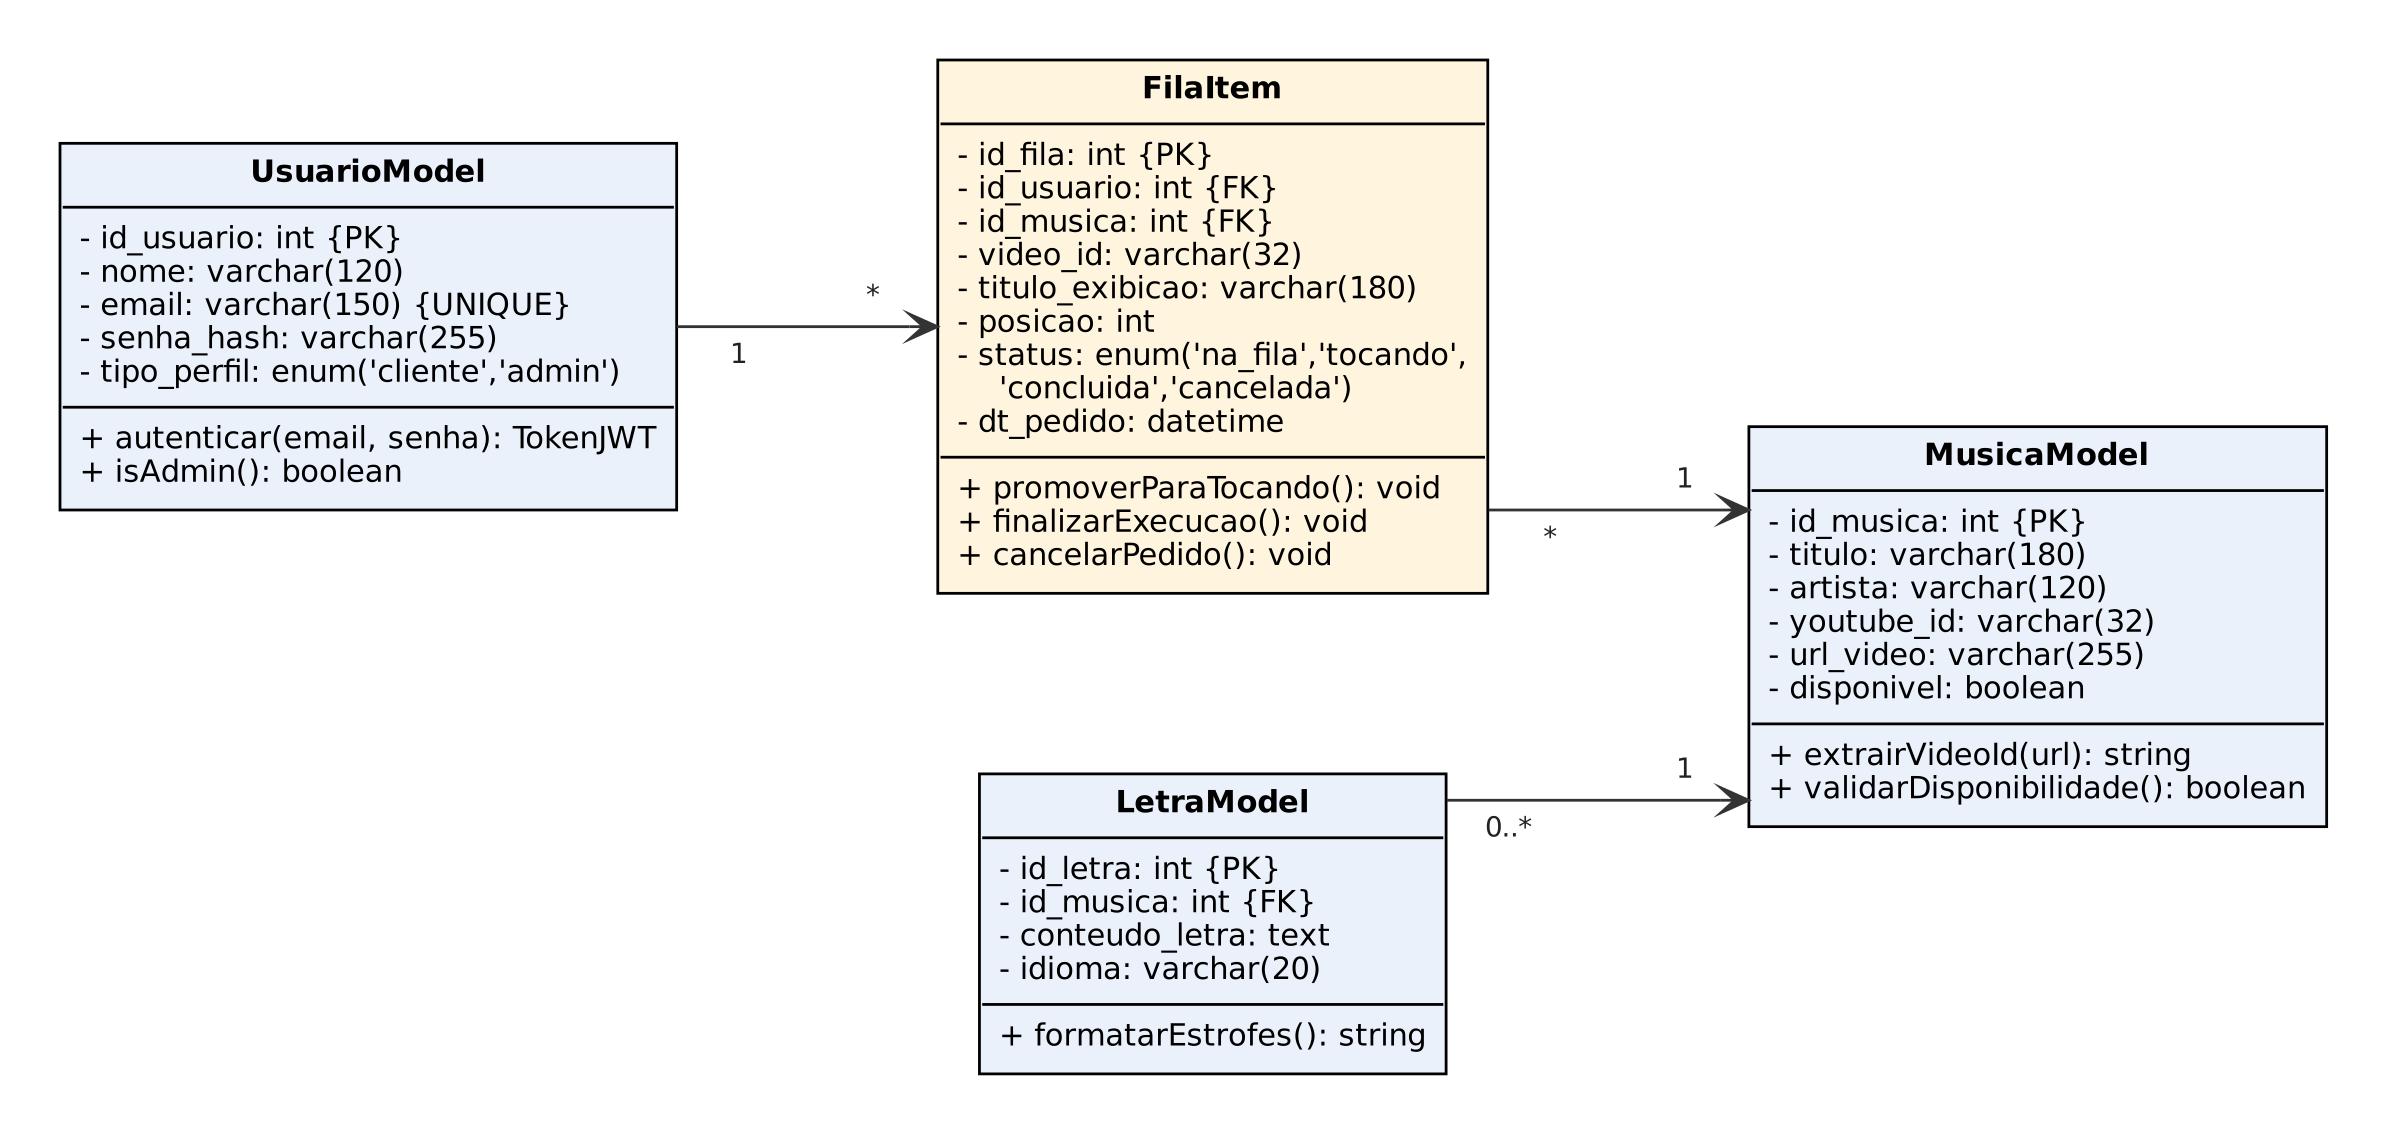
\includegraphics[width=\textwidth,height=0.78\textheight,keepaspectratio]{imagens/diagrama_classes_projeto.png}
\end{center}
\legend{Fonte: Elaborado pelos autores (2026).}
\end{caixa}

\begin{table}[H]
\IBGEtab{%
  \caption{Dicionário de dados do modelo relacional do sistema Karaokê Apache.}%
  \label{tab:dicionario_dados}%
}{%
  \footnotesize
  \begin{tabularx}{\textwidth}{p{2.0cm}p{2.9cm}p{2.7cm}p{2.0cm}X}
    \toprule
    \textbf{Tabela} & \textbf{Atributo} & \textbf{Tipo Físico} & \textbf{Restrições} & \textbf{Descrição no Projeto} \\
    \midrule
    \texttt{usuario} & \texttt{id\_usuario} & \texttt{INT} & \texttt{PK, AI} & Chave primária do usuário. \\
    \texttt{usuario} & \texttt{nome} & \texttt{VARCHAR(120)} & \texttt{NOT NULL} & Nome do participante ou operador. \\
    \texttt{usuario} & \texttt{email} & \texttt{VARCHAR(150)} & \texttt{UNIQUE} & E-mail de login do usuário. \\
    \texttt{usuario} & \texttt{senha\_hash} & \texttt{VARCHAR(255)} & \texttt{NOT NULL} & Senha criptografada (Bcrypt). \\
    \texttt{usuario} & \texttt{tipo\_perfil} & \texttt{ENUM('cliente','admin')} & \texttt{NOT NULL} & Perfil de permissão no sistema. \\
    \midrule
    \texttt{musica} & \texttt{id\_musica} & \texttt{INT} & \texttt{PK, AI} & Identificador único da música. \\
    \texttt{musica} & \texttt{titulo} & \texttt{VARCHAR(180)} & \texttt{NOT NULL} & Nome da música no catálogo. \\
    \texttt{musica} & \texttt{artista} & \texttt{VARCHAR(120)} & \texttt{NOT NULL} & Banda ou intérprete original. \\
    \texttt{musica} & \texttt{youtube\_id} & \texttt{VARCHAR(32)} & \texttt{NOT NULL} & Código de 11 caracteres do YouTube. \\
    \texttt{musica} & \texttt{url\_video} & \texttt{VARCHAR(255)} & \texttt{NOT NULL} & URL completa do vídeo de karaokê. \\
    \texttt{musica} & \texttt{disponivel} & \texttt{BOOLEAN} & \texttt{DEFAULT 1} & Indica se a música está ativa (RN00). \\
    \midrule
    \texttt{letra} & \texttt{id\_letra} & \texttt{INT} & \texttt{PK, AI} & Identificador único da letra. \\
    \texttt{letra} & \texttt{id\_musica} & \texttt{INT} & \texttt{FK, NOT NULL} & Referência à tabela \texttt{musica}. \\
    \texttt{letra} & \texttt{conteudo\_letra} & \texttt{TEXT} & \texttt{NOT NULL} & Letra completa da canção. \\
    \texttt{letra} & \texttt{idioma} & \texttt{VARCHAR(20)} & \texttt{DEFAULT 'pt-BR'} & Idioma da letra cadastrada. \\
    \midrule
    \texttt{fila} & \texttt{id\_fila} & \texttt{INT} & \texttt{PK, AI} & Identificador único do item na fila. \\
    \texttt{fila} & \texttt{id\_usuario} & \texttt{INT} & \texttt{FK, NULL} & Referência ao cliente solicitante. \\
    \texttt{fila} & \texttt{id\_musica} & \texttt{INT} & \texttt{FK, NULL} & Referência à música solicitada. \\
    \texttt{fila} & \texttt{posicao} & \texttt{INT} & \texttt{NOT NULL} & Ordem de chamada na fila ativa. \\
    \texttt{fila} & \texttt{status} & \texttt{ENUM('na\_fila', 'tocando', 'concluida', 'cancelada')} & \texttt{DEFAULT 'na\_fila'} & Estado atual do pedido (RN04). \\
    \texttt{fila} & \texttt{dt\_pedido} & \texttt{DATETIME} & \texttt{DEFAULT NOW()} & Data e hora do registro na fila. \\
    \bottomrule
  \end{tabularx}%
}{%
  \fonte{Elaborado pelos autores a partir de \texttt{Conceitual.brM3} (2026).}%
}
\end{table}

\section{Projeto da Interface do Usuário}

O projeto visual das interfaces do sistema priorizou simplicidade operacional, alto contraste em tema escuro (\textit{Dark Mode}) para uso confortável no ambiente noturno do Apache Gru Rock Bar e separação rigorosa entre a tela de controle e a tela pública do telão:

\begin{enumerate}
  \item \textbf{Interface Web de Controle e Fila (\texttt{Karaokê -- Controle e Fila}):} projetada para execução em navegador web (móvel e desktop), apresenta três blocos visuais empilhados:
    \begin{itemize}
      \item \textit{Bloco de Busca e Escolha de Vídeo:} permite ao usuário pesquisar e escolher o vídeo musical diretamente pelo próprio sistema, acionando o botão \textbf{Adicionar à fila};
      \item \textit{Card ``Tocando Agora'':} painel destacado com indicador luminoso verde em tempo real, exibindo o título e o código da música em execução no palco, acompanhado do botão \textbf{Próxima música};
      \item \textit{Lista ``Fila de Músicas (N)'':} listagem numerada sequencialmente ($1, 2, \dots, N$) com botões de ação rápida para iniciar a faixa (\textbf{Play}), remover um item individual (\textbf{X}) ou acionar \textbf{Limpar fila}.
    \end{itemize}
  \item \textbf{Interface Desktop Nativa (\texttt{Karaokê TV Player} em Electron):} projetada para exibição no telão/projetor do bar (junto ao QR Code de acesso rápido), contém uma barra de status superior minimalista (\textit{``Conectado -- Tocando: [ID\_DO\_VIDEO]''}) e dedica a área principal ao reprodutor de vídeo em tela cheia.
\end{enumerate}

O Quadro \ref{quad:interfaces_mvp} representa a disposição visual (\textit{wireframe} de projeto) das duas interfaces integradas.

\Needspace{11.7cm}
\begin{caixa}{Representação das Interfaces de Usuário (Web Controle/Fila e Electron TV Player)}{quad:interfaces_mvp}
\begin{center}
  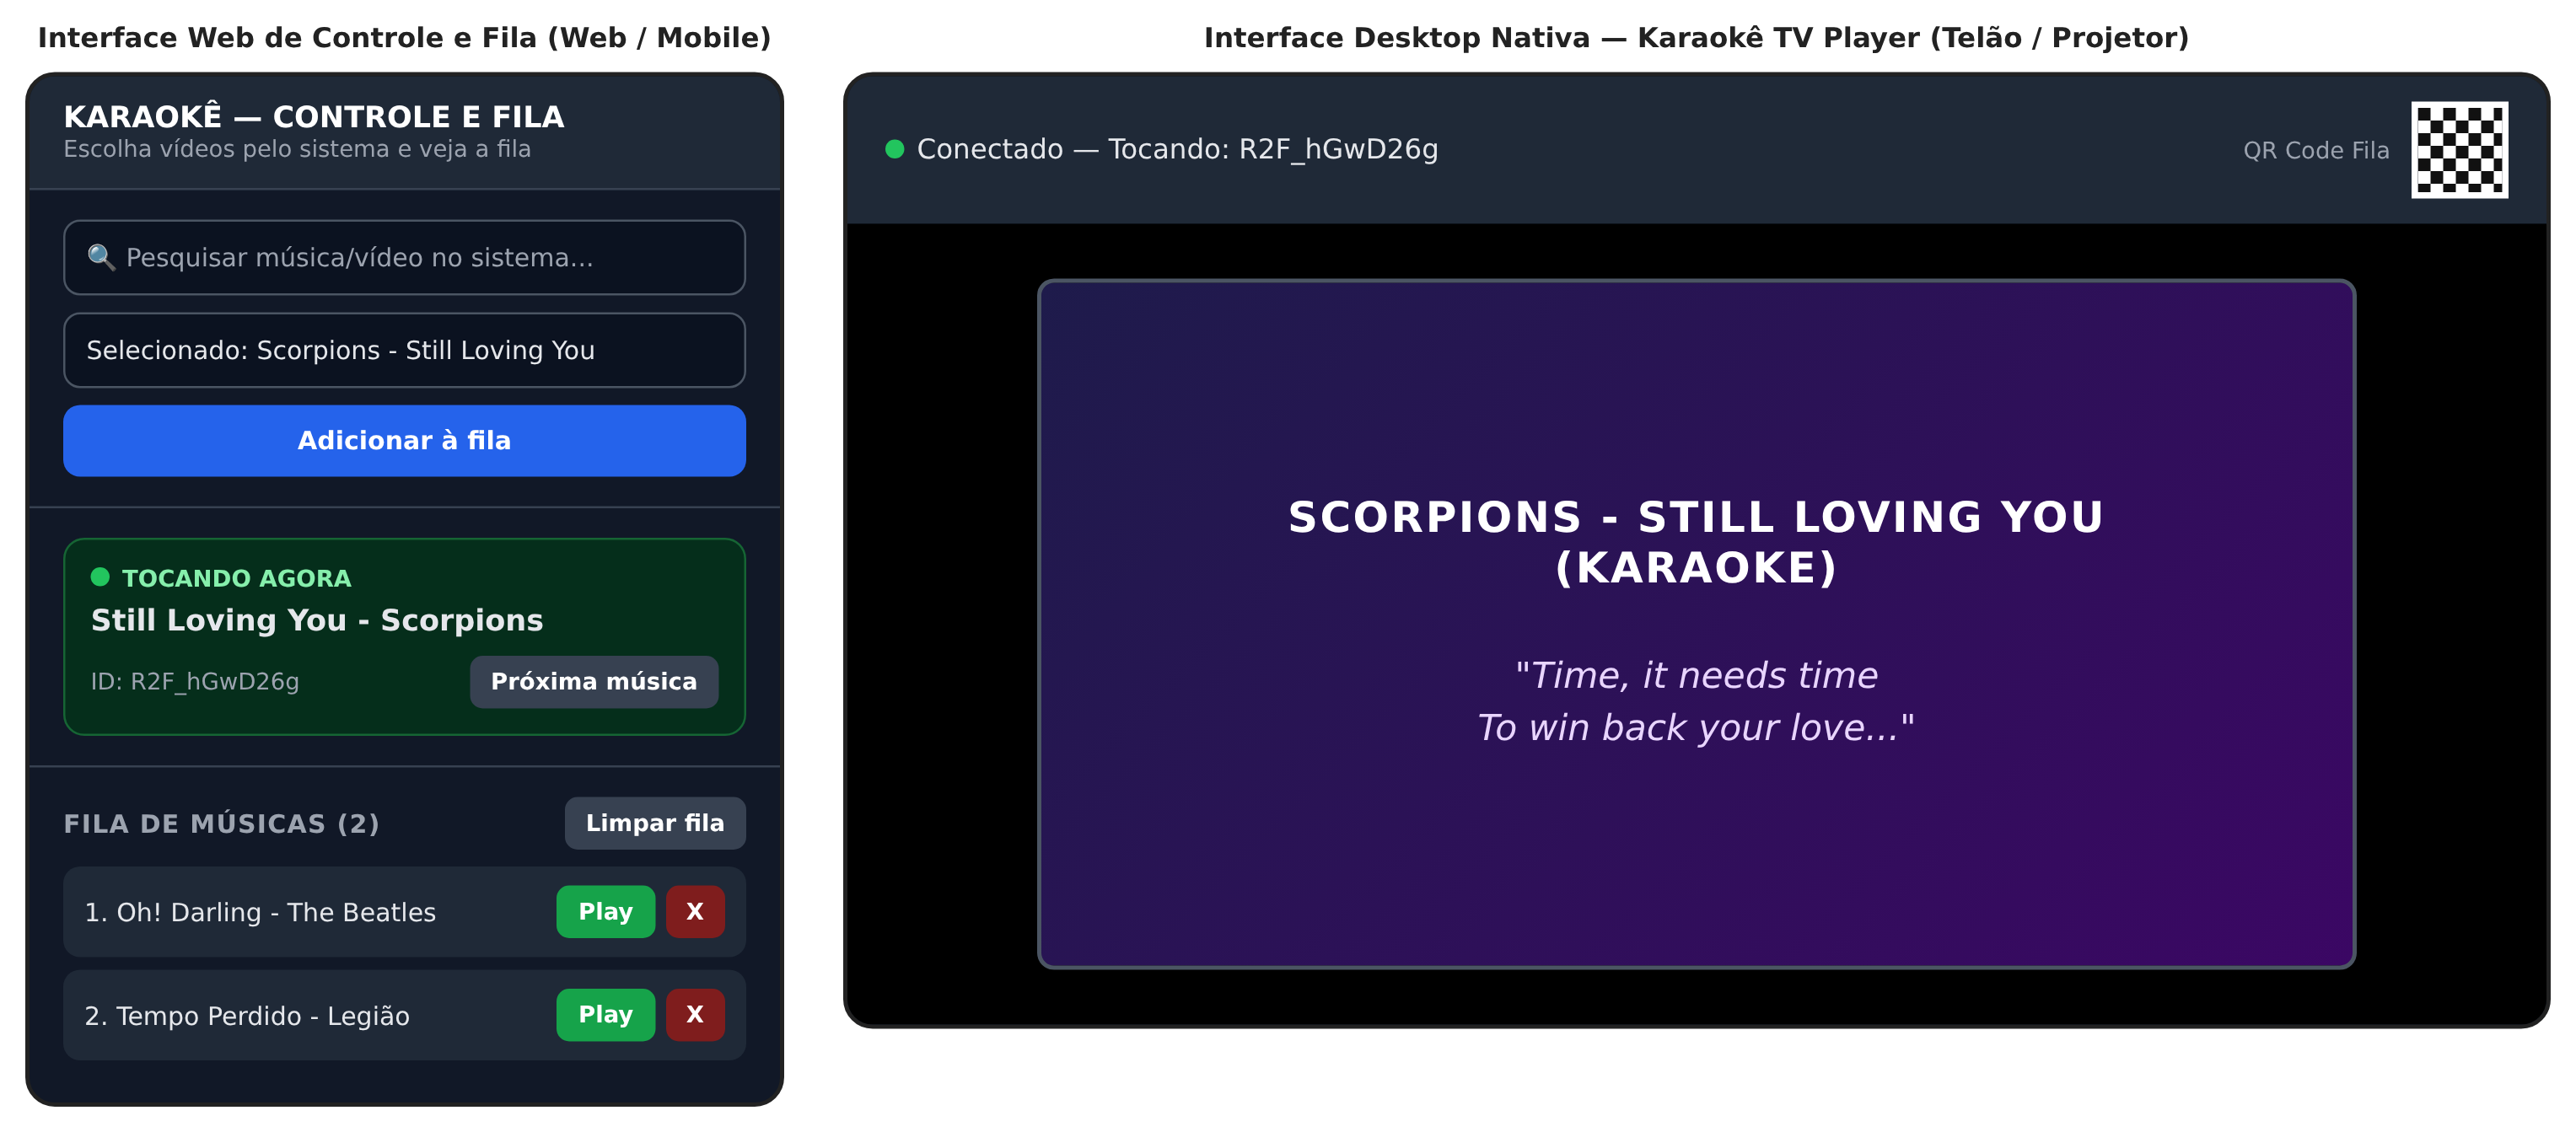
\includegraphics[width=\textwidth,height=0.78\textheight,keepaspectratio]{imagens/wireframe_interfaces.png}
\end{center}
\legend{Fonte: Elaborado pelos autores com base nas telas do projeto e \texttt{Poc.mp4} (2026).}
\end{caixa}

\section{Diagramas de Interação}

Para demonstrar como os objetos e subsistemas colaboram dinamicamente ao longo do tempo para cumprir os requisitos do sistema, o Quadro \ref{quad:sequencia} apresenta o \textbf{Diagrama de Sequência UML} correspondente ao cenário principal de submissão de um pedido musical e seu posterior acionamento para reprodução no telão em Electron.

\Needspace{15.5cm}
\begin{caixa}{Diagrama de Sequência UML -- Submissão de Música e Sincronização com o Telão}{quad:sequencia}
\begin{center}
  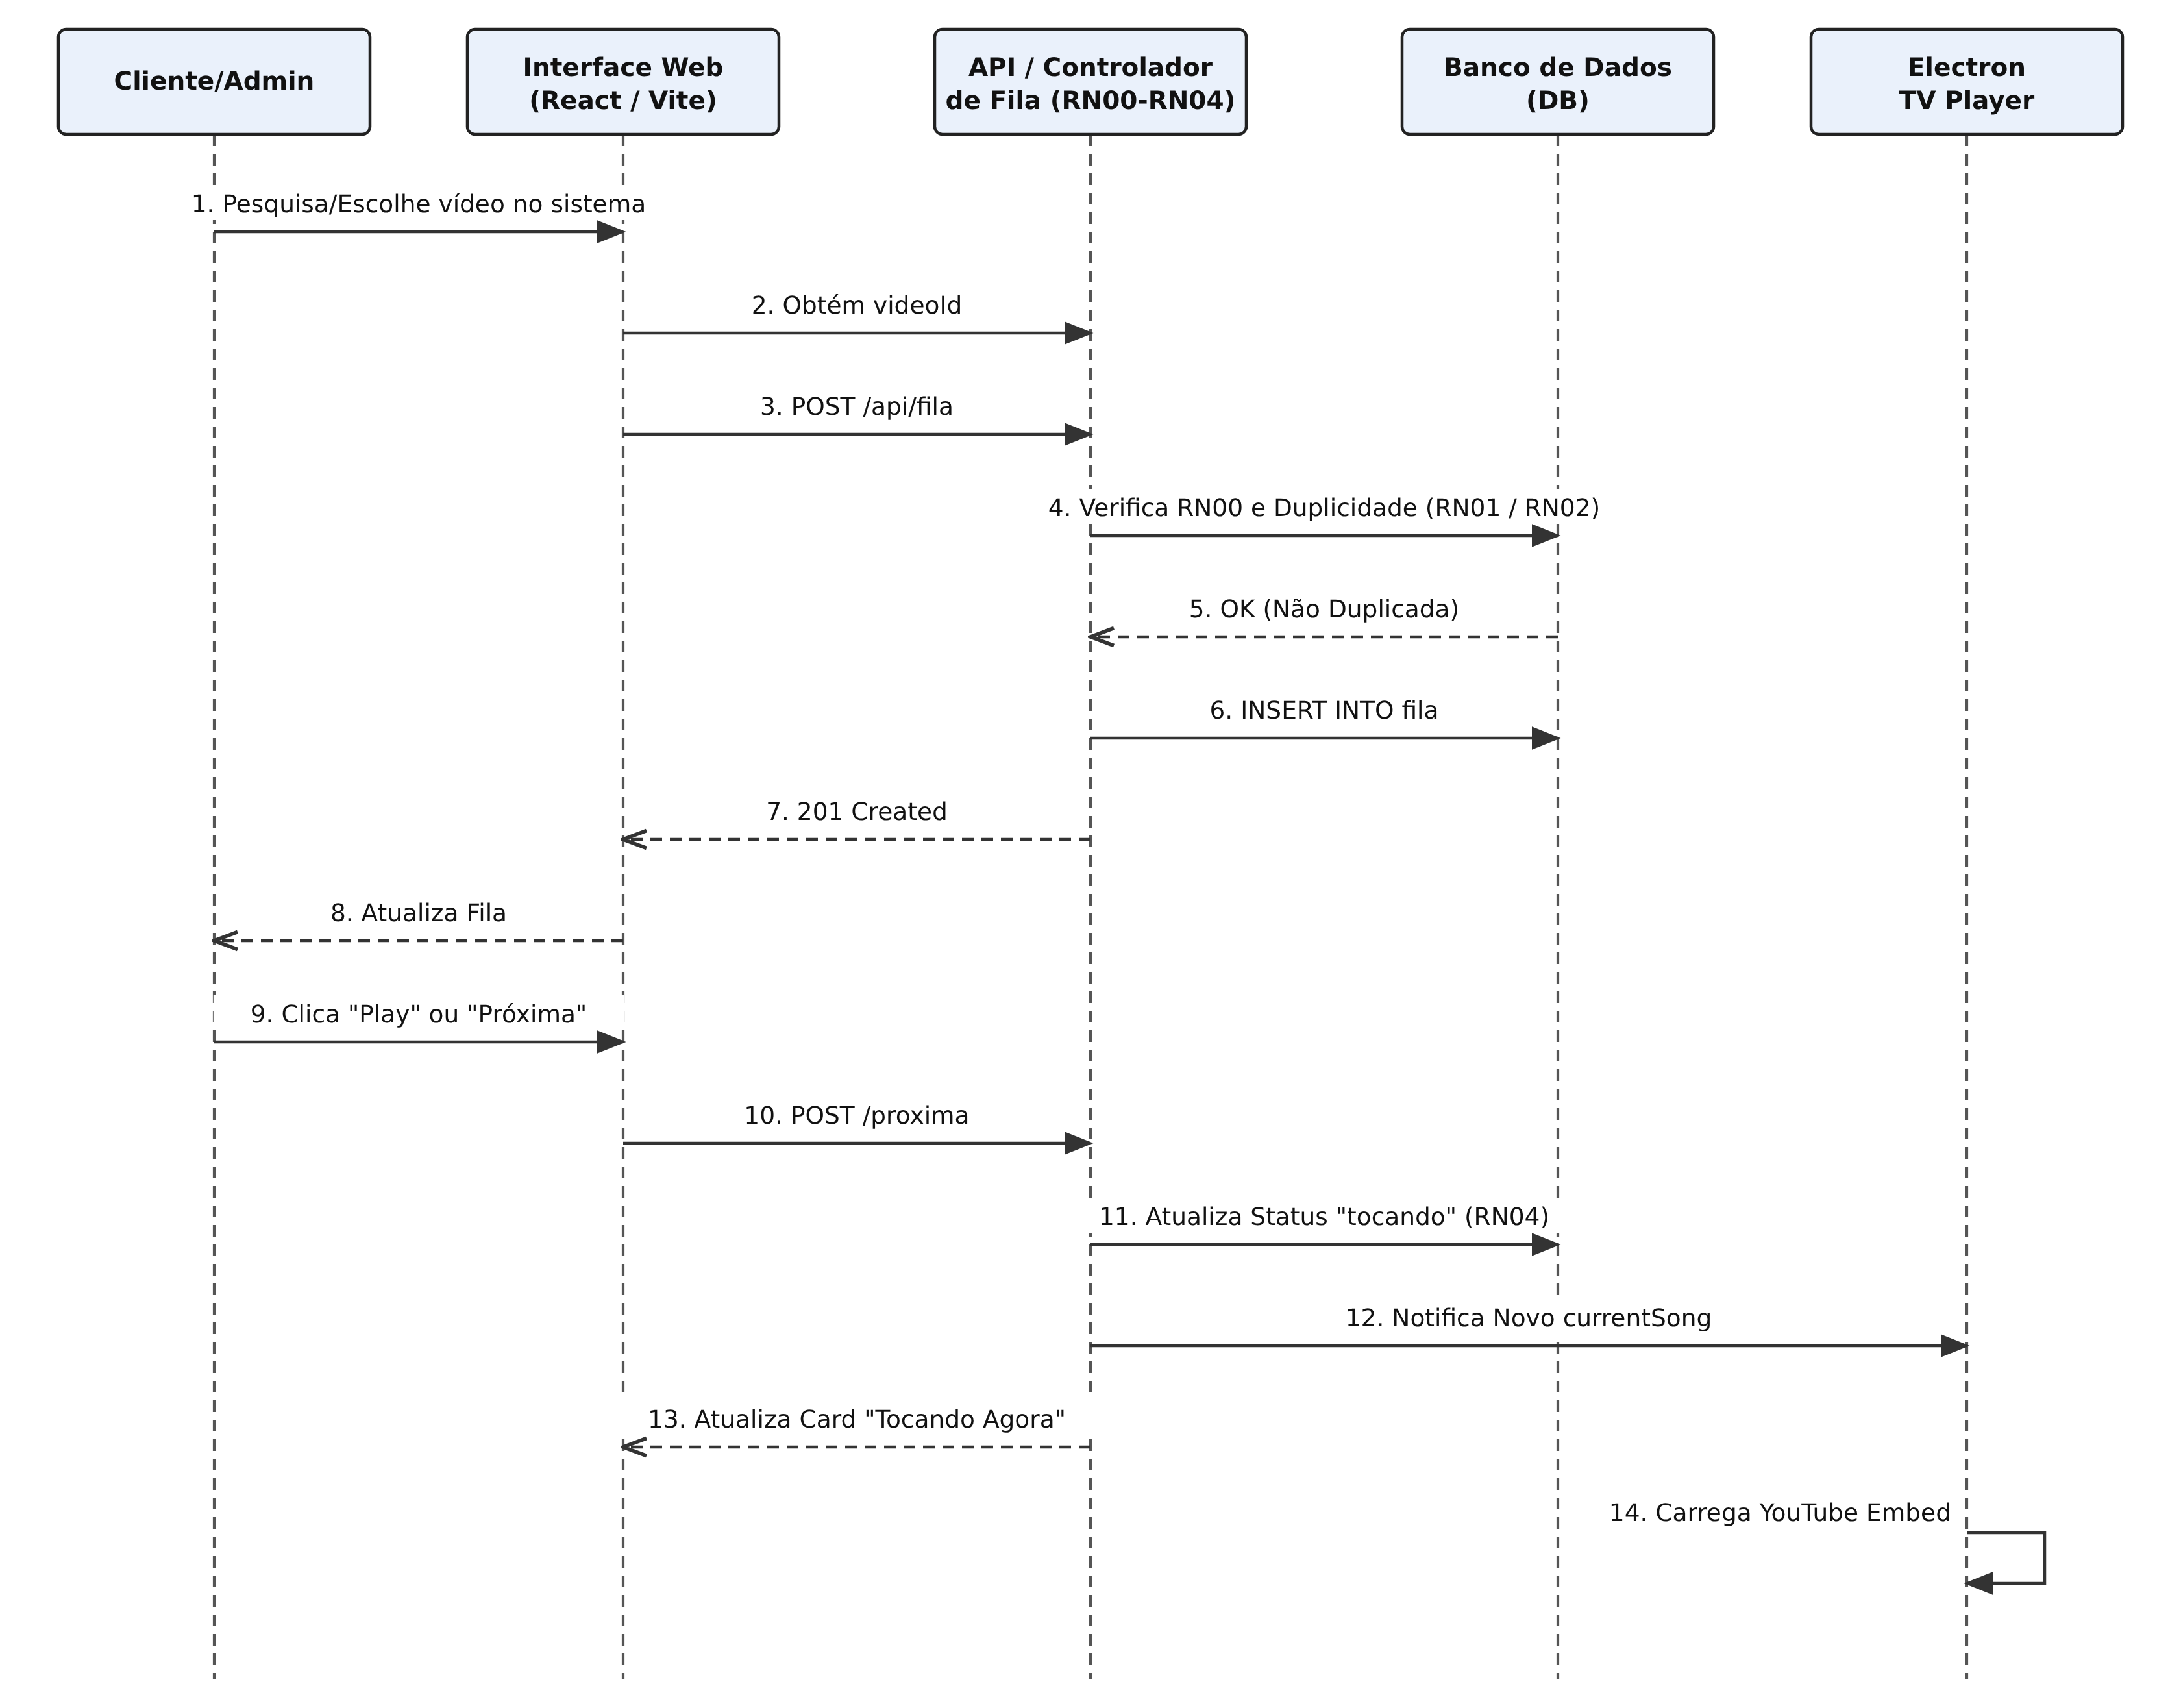
\includegraphics[width=\textwidth,height=0.78\textheight,keepaspectratio]{imagens/diagrama_sequencia.png}
\end{center}
\legend{Fonte: Elaborado pelos autores (2026).}
\end{caixa}

\section{Tecnologias Utilizadas}

A seleção tecnológica do projeto priorizou ferramentas modernas, multiplataforma e amplamente adotadas pelo mercado de desenvolvimento de software, consolidadas na Tabela \ref{tab:tecnologias}.

\begin{table}[H]
\IBGEtab{%
  \caption{Tecnologias, frameworks e ferramentas utilizadas no projeto.}%
  \label{tab:tecnologias}%
}{%
  \footnotesize
  \begin{tabularx}{\textwidth}{p{3.2cm}p{3.4cm}X}
    \toprule
    \textbf{Categoria} & \textbf{Tecnologia / Ferramenta} & \textbf{Função Desempenhada no Projeto} \\
    \midrule
    Front-end Web & React 19 + Vite \cite{react2025} & Construção reativa da interface de controle e fila (\textit{Single Page Application}), com atualização instantânea de estado e empacotamento rápido via Vite. \\
    \addlinespace
    Aplicação Desktop (Telão) & Electron \cite{electron2025} & Encapsulamento nativo do reprodutor \textit{Karaokê TV Player}, garantindo execução dedicada em tela cheia, controle de políticas de rede e isolamento de contexto. \\
    \addlinespace
    Back-end / API Orquestradora & Java 21 & Desenvolvimento da API RESTful centralizada, aplicação das regras de negócio (RN00--RN04), autenticação e orquestração da fila de reprodução. \\
    \addlinespace
    Banco de Dados & MySQL & Sistema de Gerenciamento de Banco de Dados relacional utilizado para a persistência estruturada das tabelas \texttt{usuario}, \texttt{musica}, \texttt{letra} e \texttt{fila} conforme modelado no arquivo \texttt{Conceitual.brM3}. \\
    \addlinespace
    Modelagem de Engenharia & brModelo, UMLet (\texttt{.uxf}) e Draw.io & Construção do Modelo Entidade-Relacionamento conceitual e dos diagramas arquiteturais e UML do sistema. \\
    \addlinespace
    Versionamento de Código & Git e GitHub & Controle de versão distribuído e colaboração entre os integrantes da equipe no repositório do projeto (\texttt{MurilloAssis/Projeto-Extensao-Karaoke}). \\
    \addlinespace
    Gestão e Documentação & Trello e \LaTeX\ / Overleaf & Acompanhamento das tarefas ágeis em quadro Kanban e editoração científica do relatório segundo as normas da ABNT. \\
    \bottomrule
  \end{tabularx}%
}{%
  \fonte{Elaborado pelos autores (2026).}%
}
\end{table}

\section{Segurança e Controle de Acesso}

O projeto de segurança e controle de acesso do sistema contempla quatro camadas de proteção, alinhadas às boas práticas de desenvolvimento seguro e à Lei Geral de Proteção de Dados Pessoais -- LGPD (Lei n{\textordmasculine} 13.709/2018) \cite{brasil2018lgpd}:

\begin{enumerate}
  \item \textbf{Autenticação e Controle de Acesso Baseado em Papéis (RBAC):} distinção entre sessões de \texttt{cliente} (autorizadas apenas a consultar o catálogo/fila e submeter pedidos sob as regras RN00--RN02) e sessões de \texttt{admin} (autorizadas a controlar a reprodução do palco conforme a RN03), utilizando senhas com hash \texttt{bcrypt} e tokens JWT;
  \item \textbf{Segurança no Processo Electron (\textit{Context Isolation} e CSP):} configuração da janela do \textit{Karaokê TV Player} com \texttt{contextIsolation: true}, \texttt{nodeIntegration: false} e diretivas estritas de \textit{Content Security Policy} (CSP) que limitam a origem de scripts e quadros (\texttt{frame-src}) exclusivamente à aplicação local e ao domínio oficial de incorporação do YouTube;
  \item \textbf{Isolamento de Variáveis de Ambiente e Credenciais de Banco:} armazenamento das credenciais de conexão ao MySQL e chaves de assinatura em variáveis de ambiente isoladas do código-fonte via \texttt{.gitignore};
  \item \textbf{Minimização de Dados (Art. 6{\textordmasculine} da LGPD):} coleta restrita ao nome de chamada ao palco e e-mail de identificação do participante.
\end{enumerate}

O Quadro \ref{quad:estados} apresenta o \textbf{Diagrama de Estados UML} que formaliza as transições de estado permitidas para um pedido musical dentro da fila (RN04) e as guardas de autorização (RN03) exigidas em cada transição.

\Needspace{20cm}
\begin{caixa}{Diagrama de Estados UML -- Ciclo de Vida de um Pedido Musical na Fila (RN03 e RN04)}{quad:estados}
\begin{center}
  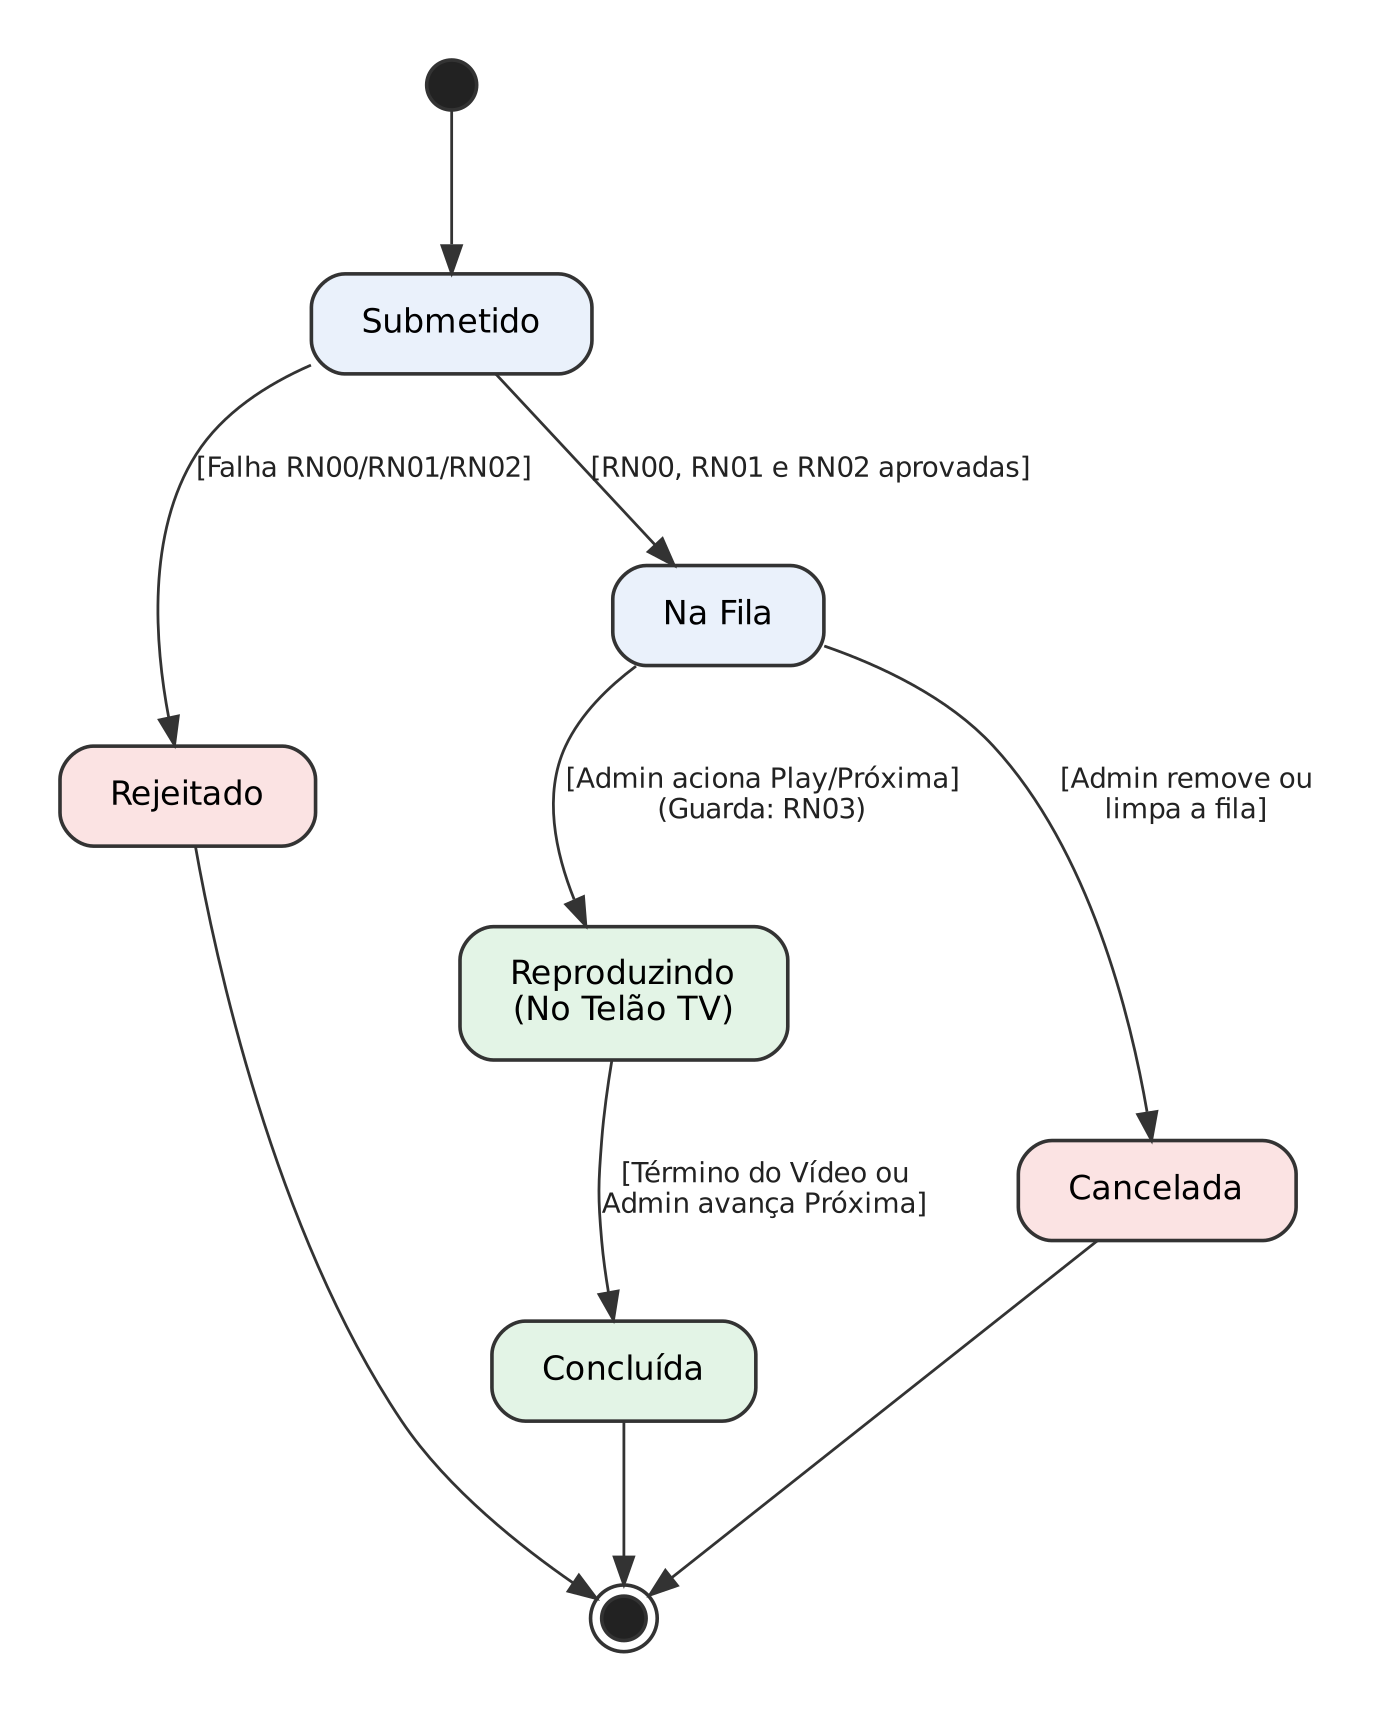
\includegraphics[width=\textwidth,height=0.78\textheight,keepaspectratio]{imagens/diagrama_estados.png}
\end{center}
\legend{Fonte: Elaborado pelos autores (2026).}
\end{caixa}

%% -------------------------------------------------------------------------- %%
